\documentclass{beamer}
\usetheme{IITIS}

% diagrams
\usepackage{tikz}
\usetikzlibrary{shapes,arrows}


\title{Introduction to quantum programming}
\author{Jaros\l aw Miszczak\\ IITiS PAN, Gliwice}
\date{April 27, 2018\\ QIPLSIGML---Machine Learning meets Quantum Computation}

\begin{document}
\begin{frame}{}
   \maketitle 
\end{frame}

%%%%%%%%%%%%%%%%%%%%%%%%%%%%%%%%%%%%%%%%%%%%%%%%%%%%%%%%%%%%%%%%%%%%%%%%%%%%%%
\begin{frame}{}
%  \tableofcontents[hideallsubsections]
    \tableofcontents
\end{frame}




%%%%%%%%%%%%%%%%%%%%%%%%%%%%%%%%%%%%%%%%%%%%%%%%%%%%%%%%%%%%%%%%%%%%%%%%%%%%%%
\section{Where are quantum computers?}
%%%%%%%%%%%%%%%%%%%%%%%%%%%%%%%%%%%%%%%%%%%%%%%%%%%%%%%%%%%%%%%%%%%%%%%%%%%%%%

%%%%%%%%%%%%%%%%%%%%%%%%%%%%%%%%%%%%%%%%%%%%%%%%%%%%%%%%%%%%%%%%%%%%%%%%%%%%%%
\begin{frame}{\insertsection}
    \begin{itemize}
        \item D-Wave (GOTO: Andy Mason and Sheir Yarkoni, Tutorial on 
        programming the D-Wave system) 
        \item IBM (GOTO: Ram Du\v{s}i\'c Hren, IBM Q Experience: Hands-on 
        workshop)
        \item Rigetti (Quil language embedded in Python)
        \item ProjectQ -- various backbends: simulator, resource counter, 
        hardware (IBM Q Experience)
    \end{itemize}
\end{frame}

%%%%%%%%%%%%%%%%%%%%%%%%%%%%%%%%%%%%%%%%%%%%%%%%%%%%%%%%%%%%%%%%%%%%%%%%%%%%%%
\section{How to use quantum computers?}
%%%%%%%%%%%%%%%%%%%%%%%%%%%%%%%%%%%%%%%%%%%%%%%%%%%%%%%%%%%%%%%%%%%%%%%%%%%%%%

%%%%%%%%%%%%%%%%%%%%%%%%%%%%%%%%%%%%%%%%%%%%%%%%%%%%%%%%%%%%%%%%%%%%%%%%%%%%%%
\begin{frame}{\insertsection}

  \begin{itemize}
    \item Level 0: Direct usage of quantum gates
        \begin{itemize}
            \item Visual manipulation of gates and circuits
            \item Multiplication of matrices and vectors 
        \end{itemize}
    \item Level 1: Embedded language with data abstraction and classical 
    control of quantum memory
    \item Level 2: Domain specific language with data and function abstraction
        \begin{itemize}
            \item QCL
            \item LanQ
        \end{itemize}
  \end{itemize}
\end{frame}


%%%%%%%%%%%%%%%%%%%%%%%%%%%%%%%%%%%%%%%%%%%%%%%%%%%%%%%%%%%%%%%%%%%%%%%%%%%%%%
\subsection{Direct usage of quantum gates}
%%%%%%%%%%%%%%%%%%%%%%%%%%%%%%%%%%%%%%%%%%%%%%%%%%%%%%%%%%%%%%%%%%%%%%%%%%%%%%
\begin{frame}{\insertsection}{\insertsubsection}
    \begin{itemize}
    \item IBM Q Experience: 
    {\small\url{https://quantumexperience.ng.bluemix.net/qx/editor}}
    \item Packages/matrix manipulation libraries:
    \begin{itemize}
        \item quantum-octave: 
        {\small \url{https://github.com/ZKSI/quantum-octave}}
        \item QuTiP: {\small\url{http://qutip.org/}}
        \item Quipper: 
        {\small\url{https://www.mathstat.dal.ca/~selinger/quipper/}}
    \end{itemize}
    \end{itemize}

\end{frame}

%%%%%%%%%%%%%%%%%%%%%%%%%%%%%%%%%%%%%%%%%%%%%%%%%%%%%%%%%%%%%%%%%%%%%%%%%%%%%%
\section{QRAM model}
%%%%%%%%%%%%%%%%%%%%%%%%%%%%%%%%%%%%%%%%%%%%%%%%%%%%%%%%%%%%%%%%%%%%%%%%%%%%%%

%%%%%%%%%%%%%%%%%%%%%%%%%%%%%%%%%%%%%%%%%%%%%%%%%%%%%%%%%%%%%%%%%%%%%%%%%%%%%%
\subsection{Data abstraction and classical control of quantum memory}
%%%%%%%%%%%%%%%%%%%%%%%%%%%%%%%%%%%%%%%%%%%%%%%%%%%%%%%%%%%%%%%%%%%%%%%%%%%%%%
\begin{frame}{\insertsection}{\insertsubsection}
    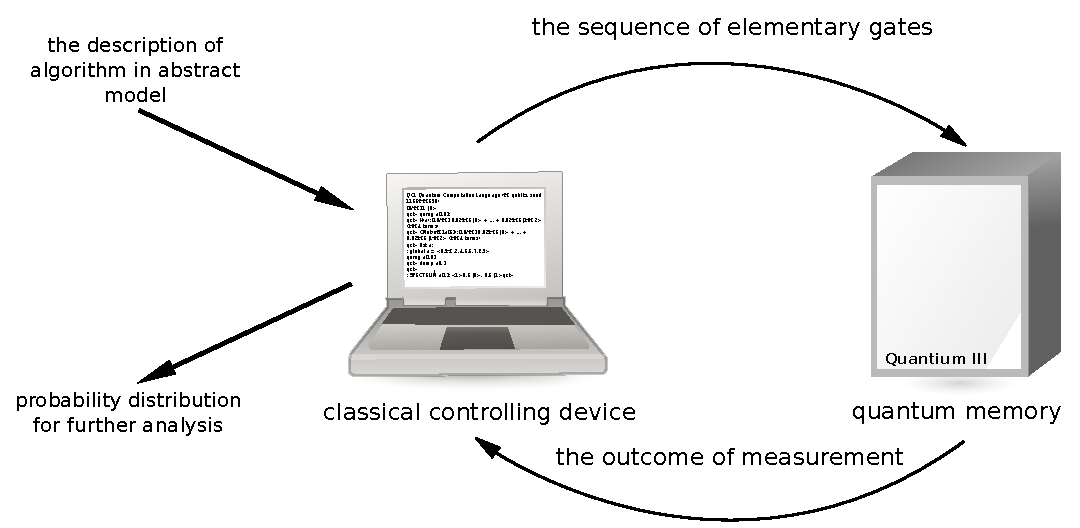
\includegraphics[width=\textwidth]{pics/qram}
\end{frame}


%%%%%%%%%%%%%%%%%%%%%%%%%%%%%%%%%%%%%%%%%%%%%%%%%%%%%%%%%%%%%%%%%%%%%%%%%%%%%%
\subsection{Software architecture}
%%%%%%%%%%%%%%%%%%%%%%%%%%%%%%%%%%%%%%%%%%%%%%%%%%%%%%%%%%%%%%%%%%%%%%%%%%%%%%
%%%%%%%%%%%%%%%%%%%%%%%%%%%%%%%%%%%%%%%%%%%%%%%%%%%%%%%%%%%%%%%%%%%%%%%%%%%%%%
\begin{frame}{\insertsection}{\insertsubsection}
\centering
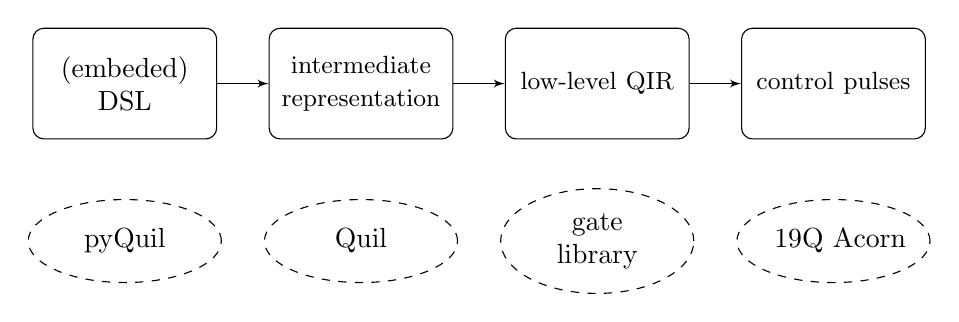
\begin{tikzpicture}[node distance = 3cm, auto]

\tikzstyle{block} = [rectangle, draw, text width=2.1cm, text centered, rounded 
corners, minimum height=4em]
\tikzstyle{example} = [draw, ellipse, node distance=2cm,  text width=1.5cm, 
dashed,
text centered, minimum  height=3em]
\tikzstyle{line} = [draw, -latex', thin]

\node [block] (edsl) {(embeded) DSL};
\node [example, below of=edsl] (edsl-ex) {pyQuil};

\node [block, right of=edsl] (qir) {\small intermediate representation};
\node [example, below of=qir] (qir-ex) {Quil};

\node [block, right of=qir] (qoptim) {\small low-level QIR};
\node [example, below of=qoptim] (qoptim-ex) {gate library};

\node [block, right of=qoptim] (qcontrol) {\small control pulses};
\node [example, below of=qcontrol] (qcontrol-ex) {19Q~Acorn};

\path [line] (edsl) -- (qir);
\path [line] (qir) -- (qoptim);
\path [line] (qoptim) -- (qcontrol);
\end{tikzpicture}

\end{frame}


%%%%%%%%%%%%%%%%%%%%%%%%%%%%%%%%%%%%%%%%%%%%%%%%%%%%%%%%%%%%%%%%%%%%%%%%%%%%%%
\subsection{Examples}
%%%%%%%%%%%%%%%%%%%%%%%%%%%%%%%%%%%%%%%%%%%%%%%%%%%%%%%%%%%%%%%%%%%%%%%%%%%%%%



%%%%%%%%%%%%%%%%%%%%%%%%%%%%%%%%%%%%%%%%%%%%%%%%%%%%%%%%%%%%%%%%%%%%%%%%%%%%%%
\begin{frame}{}
	
\end{frame}


%%%%%%%%%%%%%%%%%%%%%%%%%%%%%%%%%%%%%%%%%%%%%%%%%%%%%%%%%%%%%%%%%%%%%%%%%%%%%%
\begin{frame}{}
	
\end{frame}


%%%%%%%%%%%%%%%%%%%%%%%%%%%%%%%%%%%%%%%%%%%%%%%%%%%%%%%%%%%%%%%%%%%%%%%%%%%%%%
\begin{frame}{}
	
\end{frame}


%%%%%%%%%%%%%%%%%%%%%%%%%%%%%%%%%%%%%%%%%%%%%%%%%%%%%%%%%%%%%%%%%%%%%%%%%%%%%%
\begin{frame}{}
	
\end{frame}


%%%%%%%%%%%%%%%%%%%%%%%%%%%%%%%%%%%%%%%%%%%%%%%%%%%%%%%%%%%%%%%%%%%%%%%%%%%%%%
\begin{frame}{}
	
\end{frame}


%%%%%%%%%%%%%%%%%%%%%%%%%%%%%%%%%%%%%%%%%%%%%%%%%%%%%%%%%%%%%%%%%%%%%%%%%%%%%%
\begin{frame}{}
	
\end{frame}


%%%%%%%%%%%%%%%%%%%%%%%%%%%%%%%%%%%%%%%%%%%%%%%%%%%%%%%%%%%%%%%%%%%%%%%%%%%%%%
\begin{frame}{}
	
\end{frame}






\end{document}
